\chapter{Wykorzystane biblioteki i narzędzia}

W rozdziale tym opisano krótko biblioteki oraz narzędzia wykorzystane podczas realizacji pracy magisterskiej do weryfikacji wytycznych klinicznych oraz do implementacji systemu wspomagania decyzji klinicznych. 

\section{ECLiPSe}
\label{sec:eclipse}

System ECLiPSe \cite{EclipseSite} środowiskiem do tworzenia i wykonywania programów CLP. Jest ono udostępniane na licencji \textit{open source} i może działać na wielu systemach operacyjnych. Główne okno systemu ECLiPSe zostało przedstawione na rys. \ref{fig:eclipse}. Składa się ono z trzech części. Pierwsza część służy do edycji programów (mogą zostać one odczytane z zewnętrznych plików źródłowych i skompilowane -- przykładowy program przedstawiono na rys. \ref{fig:sendmoremoney}), druga część okna wyświetla wyniki, trzecia natomiast pokazuje ewentualne błędy oraz inne komunikaty.
 
\begin{figure}[H]
\centering
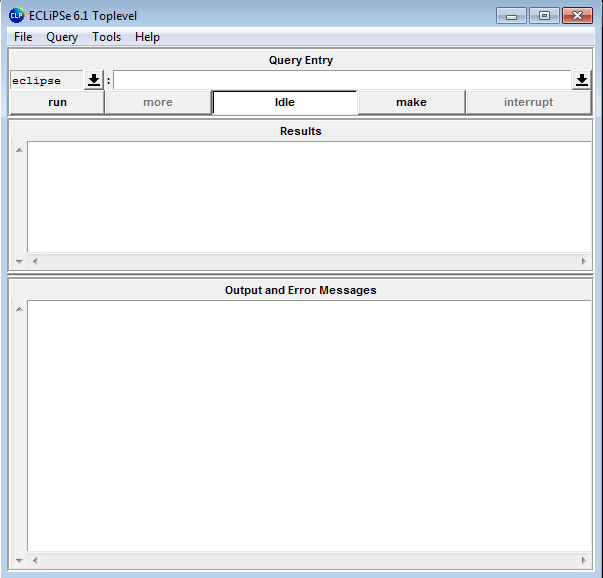
\includegraphics[width=0.7\textwidth]{img/okno.png}
\caption{Główne okno systemu ECLiPSe}
\label{fig:eclipse}
\end{figure}

W niniejszej pracy system ECliPSe został użyty do testowania przykładowych wytycznych medycznych. Nie współpracuje on natomiast ze zrealizowanym systemem wspomagania decyzji klinicznych -- do tego celu wykorzystano system Choco 3 opisany w kolejnym punkcie. 

\section{Choco 3}


Choco 3 \cite{Choco3} jest darmową biblioteką w języku Java (wersja 8), która pozwala na rozwiązywanie problemów CLP. Podobnie jak system ECLiPSe, jest ona udostępniana jako \textit{open source}.

Główną klasą biblioteki jest klasa \texttt{Solver}. Do obiektu z tej klasy  można dołączyć zmienną (klasa \texttt{IntVar}) podając obiekt \texttt{Solver-a} w ostatnim argumencie metody \texttt{VariableFactory.bounded}. Pozostałe argumenty tej metody to nazwa zmiennej oraz dolne i górne ograniczenie zmiennej. W pracy magisterskiej wykorzystywane są w większości zmienne, dla których dolne ograniczenie jest równe 0, a górne ograniczenie jest równe 1, czyli są to zmienne przyjmujące wartości prawda/fałsz. Za pomocą metody \texttt{Solver.post} można dodawać nowe ograniczenia. Ograniczenia tworzy się m.in. za pomocą klasy \texttt{IntConstraintFactory}. Jedną z podstawowych metod tworzących ograniczenia jest funkcja \texttt{arithm}. Przykładowo, można za jej pomocą określić, że suma dwóch zmiennych X i Y ma być mniejsza od 5. Po określeniu ograniczeń można uruchomić \texttt{Solver} i wygenerować rozwiązanie za pomocą metody \texttt{findSolution}. Kolejne rozwiązania można uzyskać za pomocą metody \texttt{nextSolution}. Odczytanie wartości zmiennej określonego rozwiązania polega na wywołaniu metody \texttt{IntVar.getValue}. 

Na rys. \ref{fig:choco} przedstawiono prosty program dla Choco 3 szukający takich zmiennych X i Y (są to zmienne przyjmujące wartości 0 lub 1), których suma jest równa 1. Problem ten posiada dwa rozwiąnia: X=1, Y=0 oraz X=0, Y=1.

\begin{figure}
\begin{verbatim}
Solver solver = new Solver("my first problem");
IntVar x = VariableFactory.bounded("X", 0, 1, solver);
IntVar y = VariableFactory.bounded("Y", 0, 1, solver);
solver.post(IntConstraintFactory.arithm(x, "+", y, "=", 1));
solver.findSolution();
do {
   System.out.println("X="+x.getValue()+", Y="+y.getValue());
} while(solver.nextSolution());
\end{verbatim}
\caption{Przykładowy program CLP dla biblioteki Choco 3}
\label{fig:choco}
\end{figure}

\section{Graphviz}

Graphviz \cite{Graphviz} jest pakietem narzędzi służących do wizualizacji grafów. Pozwala na konwersję pliku tekstowego w formacie DOT do obrazu przedstawiającego graf. Program automatycznie rozmieszcza wierzchołki grafu -- nie jest konieczne podawanie ich współrzędnych. Ponadto program automatycznie rysuje krawędzie tak, aby ograniczyć liczbę ich przecięć. 

W skład pakietu wchodzi również program \texttt{gvedit}, który jest programem okienkowym pozwalającym na weryfikację i wizualizację plików w formacie DOT. Po otwarciu takiego pliku wypisywana jest lista błędów, które należy poprawić (jeśli plik jest niepoprawny), albo wyświetlany jest obraz przedstawiający graf. Podobną funkcjonalność ma program \texttt{dot}, z tą różnicą, że jest to program konsolowy (bez graficznego interfejsu użytkownika). Program \texttt{dot} przyjmuje 3 parametry. Pierwszym argumentem jest ścieżka do pliku w formacie DOT, drugim jest format generowanego obrazu (przykładowo dla uzyskania formatu PNG obrazka podajemy drugi parametr równy \texttt{–Tpng}). Trzeci parametr poprzedzony jest przełącznikiem \texttt{-o} i jest to ścieżka do wynikowego obrazu. 

Składnia pliku w formacie DOT jest następująca. Na początku pliku znajduje się słowo \texttt{digraph}, po którym umieszcza się nazwę grafu. Wszystkie pozostałe właściwości grafu są umieszczone w bloku otoczonym nawiasami klamrowymi. W bloku tym można podać globalne atrybuty dla wierzchołków oraz krawędzi. Atrybuty dla wierzchołków mogą być podane po słowie \texttt{node} w bloku otoczonym nawiasami kwadratowymi, atrybuty są oddzielone od siebie przecinkami. Do przykładowych globalnych atrybutów węzłów należą m. in. kształt (\texttt{box} – prostokąt, \texttt{circle} – koło, \texttt{diamond} – romb), kolor wypełnienia, kolor konturu, grubość linii konturu, rodzaj czcionki, wielkość czcionki. Jeśli chodzi o globalne atrybuty krawędzi, to można je podać w podobny sposób jak globalne atrybuty węzłów, z tą różnicą, że zamiast słowa \texttt{node} należy podać słowo \texttt{edge}. Można też określić atrybuty globalne dla całego grafu -- do nich należą przede wszystkim wielkość i rodzaj czcionki (krawędzie mogą posiadać etykiety). 

Następnie podaje się wierzchołki i krawędzie z ich unikalnymi atrybutami. Atrybut pojedynczego węzła lub krawędzi, jeśli już wystąpił w globalnych atrybutach węzłów lub krawędzi, zostaje nadpisany przez wersję lokalną. Opis pojedynczego węzła polega na podaniu jego unikalnego identyfikatora, a następnie jego atrybutów w bloku otoczonym nawiasami kwadratowymi.  Krawędzie natomiast tworzy się podając na początku identyfikator węzła źródłowego krawędzi, następnie wstawia się strzałkę (\texttt{->}), a na końcu identyfikator węzła docelowego. Po podaniu tych elementów można podać atrybuty krawędzi, przede wszystkim etykietę. Co ciekawe, krawędź może być także nieskierowana, wtedy zamiast strzałki (\texttt{->}) należy umieścić podwójną kreskę (\texttt{--}). 

Na rys. \ref{fig:dot_example} zaprezentowano bardzo prosty przykład pliku w formacie DOT, a na rys. \ref{fig:dot_graph} graf wygenerowany na podstawie tego pliku.

\begin{figure}
\begin{verbatim}
digraph graf{
    node [shape=box, style=filled, fillcolor=green];
    A [label="Wierzchołek A"];
    B [label="Wierzchołek B"];
    C [label="Wierzchołek C"];
    A->B;
    A->C;
}
\end{verbatim}
\caption{Prosty plik w formacie DOT}
\label{fig:dot_example}
\end{figure}


\begin{figure}[H]
\begin{center}
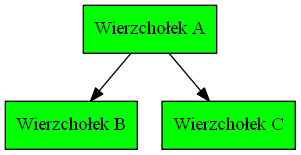
\includegraphics[width=0.3\textwidth]{img/graf.png}
\end{center}
\caption{Graf wygenerowany na podstawie pliku z rys. \ref{fig:dot_example}}
\label{fig:dot_graph}
\end{figure}

\section{JPGD}

Biblioteka JPGD (a Java parser for Graphviz documents) \cite{JPGD} służy do tworzenia obiektowej reprezentacji pliku w formacie DOT -- obiektu klasy \texttt{Graph} posiadającego listę obiektów klasy \texttt{Node} oraz \texttt{Edge}. Do konwersji wykorzystywany jest obiekt klasy \texttt{Parser}. Klasa \texttt{Parser} posiada funkcję \texttt{parse}, której konstruktor jako parametr przyjmuje obiekt klasy \texttt{FileReader} odwołujący się do określonego pliku DOT. Listę odczytanych grafów można uzyskać za pomocą metody \texttt{Parser.getGraphs}.

Wierzchołki grafu można pozyskać za pomocą metody \texttt{Graph.getNodes}, natomiast  krawędzie grafu za pomocą \texttt{Graph.getEdges}. Wierzchołki i oraz krawędzie posiadają atrybuty. Do atrybutów wierzchołka należy etykieta, kształt, kolor wypełnienia, kolor konturu i grubość linii konturu. Krawędzie posiadają przede wszystkim jeden istotny atrybut -– etykietę. Wartości wszystkich tych atrybutów można odczytać za pomocą metody \texttt{getAttribute}, której argumentem jest nazwa atrybutu. Natomiast ustawienie  wartości atrybutu odbywa się za pomocą metody \texttt{setAttribute}, której pierwszym argumentem jest nazwa atrybutu, a drugim jego wartość. 

Każdy wierzchołek grafu zapisanego w formacie DOT posiada także swój unikalny identyfikator. Identyfikatory przechowywane są jako obiekty klasy \texttt{Id}. Można je uzyskać wywołując metodę \texttt{Node.getId}. Ponowne wywołanie metody \texttt{getId}, w tym przypadku dla obiektu klasy \texttt{Id} daje dostęp do rzeczywistego identyfikatora węzła typu \texttt{String}. 

Dla krawędzie istnieje możliwość odczytania wierzchołka źródłowego (początkowego) oraz docelowego (końcowego). Jest to możliwe dzięki metodom \texttt{Edge.getSource} (dla uzyskania węzła źródłowego) oraz \texttt{Edge.getTarget} (dla uzyskania węzła docelowego). Obie metody zwracają obiekty klasy \texttt{PortNode}, z którego następnie możemy uzyskać obiekt klasy \texttt{Node} za pomocą metody \texttt{getNode}. Ważną metodą jest też \texttt{Graph.toString}. Pozwala ona na uzyskanie zaktualizowanego grafu w formacie DOT, uwzględniającego zmiany wprowadzone za pomocą metody \texttt{setAttribute} dla obiektów klasy \texttt{Node} lub \texttt{Edge}. 

Na rys. \ref{fig:jgpd} przedstawiono przykładowy kod źródłowy ilustrujący wykorzystanie biblioteki JPGD do znalezienia krawędzi wyjściowych węzła n.

\begin{figure}
\begin{verbatim}
public static ArrayList<Edge> getOutEdges(Graph graph, Node n) {
    ArrayList<Edge> list = new ArrayList<Edge>();
    for(Edge e:graph.getEdges()) {
       if(e.getSource().getNode() == n)
           list.add(e);
    }
    return list;
}
\end{verbatim}
\caption{Przykład wykorzystania biblioteki JPGD}
\label{fig:jgpd}
\end{figure}

